% author: zhaofeng-shu33
% license: LPPL (LaTeX project public license)
\documentclass{ctexart}
\usepackage{hyperref}
\usepackage{mathtools}
\DeclarePairedDelimiter\norm{\lVert}{\rVert}
\DeclarePairedDelimiter\abs{\lvert}{\rvert}
\usepackage{subcaption}
\usepackage{amsthm}
\usepackage{amsfonts}
\usepackage{bm}
\usepackage{dsfont}
\newtheorem{theorem}{定理}
\newtheorem{lemma}{引理}
\theoremstyle{definition}
\newtheorem{definition}{定义}
\theoremstyle{remark}
\newtheorem{remark}{评论}
\begin{document}
\title{第一次大作业}
\author{赵丰}
\maketitle
\section{概要}
本文自己实现了k-means算法,并根据自己提出的标签差异个数以及目标函的相对差两个一致性指标对比了自己的实现和工业级实现在结果上的差异,使用 Silhouette 作图来评估聚类的好坏。通过实际实验发现 Affinity Propogation 算法各方面都比较差。最后我们将k-means 聚类算法用于图像分割的情形,了解k-means聚类算法的实际应用。


\section{k-means 标准算法描述}
给定初始$k$个中心 $m_1^{(1)},\dots,m_k^{(1)}$,k-means 算法在下面两个步骤间迭代\cite{kmeans-wiki}:
\begin{description}
\item[赋值:] $S_i^{t}=\{x_p : \norm{x_p - m_i^{(t)}}\leq \norm{x_p - m_j^{(t)}} \forall j, 1\leq j \leq k\}$
\item[更新:] $ m_i^{(t+1)} = \frac{1}{\abs{S_i^{(t)}}} \displaystyle\sum_{x_j \in S_i^{(t)}} x_j$
\end{description}
\section{k-means 标准算法分析}
\subsection{正确性}
考虑目标函数
\begin{subequations}
\begin{align}
\label{kcutgiven}f(x) &=  \sum_{i=1}^k  \sum_{x\in S_i} \norm{\bm{x}-\bm{\mu}_i}^2\\ 
\label{coorgiven}& = \sum_{j=1}^n \sum_{i=1}^k \norm{\bm{x}_j - \bm{\mu}_{i}}\mathds{1}_{\bm{x}_j \in S_i} \\
\dot\bigcup_{i=1}^k S_i & =  \{\bm{x}_1,\dots,\bm{x}_n\}\nonumber
\end{align}
\end{subequations}
希望求解最优的k-划分和k个点的坐标。该问题联合求解(全局最优解)是NP-Hard的(组合优化问题一般都有这个特征),但如果给定k-划分求解k个点的坐标,根据\eqref{kcutgiven}式,由二次函数极值的性质易得其为每个划分中各点的质心;如果给定k个点的坐标,根据\eqref{coorgiven}式,每个$\bm{x}$应归入距离最近的中心所在的类。k-means 标准算法即利用了这样的关系迭代求解出\textbf{局部最优值}。

我们考察在k-means 标准算法迭代过程中取值的变化。赋值步骤相当于k个点的坐标不动,对$S_i$进行重新划分,根据\eqref{coorgiven}式从而使得目标函数减小;更新步骤相当于划分不变,重新求解k个点的坐标,根据\eqref{kcutgiven}式从而使得目标函数减小。根据单调数列收敛的结论,算法的收敛性得到保证。注意到这里使用 $L_2$ 范数即欧氏距离才可以保证这一点,因为欧氏距离才下各划分的质心才是给定$S_i$下\eqref{kcutgiven}式的最优解。

\subsection{算法时间复杂度}
假设其主要逻辑中 两个步骤共重复迭代 $t$ 次, 赋值操作要对 $k$个集合进行,对每个集合又要把所有的数据点(设为$n$个)遍历一遍,设数据为$d$ 维,则算法复杂度为$O(tknd)$。
\subsection{实际考虑}
使用脚本编程语言实现 k-means 算法时,更新步骤可以通过调用内置矩阵运算加速,避免自己写循环。在这一点上,csdn 的某个范例\cite{kmeans-csdn}做得很不好,可能会误导初学者。但即使在用户程序中使用矩阵加速,自己实现的也只能供学习、科研目的使用。
\subsection{算法验证}\label{verification}
将自己实现的 k-means 算法与工业级的实现进行对比有多种不同的方法,这里我们采用对比数据点的标签差异的个数以及目标函数(\eqref{kcutgiven}式)的相对差两个指标。由于聚类本身的标签是相对的,我们采用对$k$个标签进行全枚举的方法寻找两种实现间最佳的匹配。

用数学的语言表示,我们给出下面的定义:
\begin{definition}[k-标签数列]
若有限长数列$\ell$ 每个位置的元素取自1到k的正整数,则称该有限长数列为k-标签数列,所有k-标签数列组成集合$S$。
\end{definition}
从排列的观点,我们知道k-全排列函数$p$是定义域和值域都是1到k的整数的集合的双射。我们可以把k-全排列函数(函数全体集合记为$P$)拓展到k-标签数列上。
\begin{definition}[作用在k-标签数列上的k-全排列函数]
设$p$是k-全排列函数,$\ell$是k-标签数列,定义$\tilde{p}:S\to S,p(\ell)=\ell'$, 其中$\ell'(i)=p(\ell(i))$. $\tilde{p}$称为由$p$诱导出来的作用在k-标签数列上的k-全排列函数。
\end{definition}
我们知道离散度量$d:X\times X\to \{0,1\}$ 是空间$X$上的一种度量, 定义为 $ d(x,y)=\begin{cases}0 & x=y \\ 1 & x\neq y \end{cases}$。
$m$个数据可以看成$m$个$X$的笛卡尔乘积空间,其中$X=\{1,2,\dots,k\}$,从而$\tilde{d}: X^d \times X^d \to \{0,1\}^d,\tilde{d}(\bm{x},\bm{y})=(d(x_1,y_1), \dots, d(x_n,y_n)).$ 
\begin{definition}[聚类算法标签差异度]\label{def:label_diff}
给定两个不同实现细节的 k-means 的聚类算法,对$m$个数据进行$k$分类,标签分别为$\ell_1,\ell_2$。
标签差异度$e$定义为:
\begin{equation}
e= \frac{1}{m}\min_{p\in P} \norm{d(p(\ell_1),\ell_2)}_1
\end{equation}
\end{definition}

\begin{remark}
在定义\ref{def:label_diff}中 $d(p(\ell_1),\ell_2)$ 是$k$维向量,每个分量均为0或1,$\norm{\cdot}_1$是取$L_1$范数,即将各元素取绝对值相加。
\end{remark}


下面的定理进一步说明了聚类算法标签差异度的合理性:
\begin{theorem}\label{thm:12p}
\begin{equation}
\min_{p\in P} \norm{d(p(\ell_1),\ell_2)}_1 = \min_{q\in P} \norm{d(\ell_1,q(\ell_2))}_1 = \min_{p,q\in P} \norm{d(p(\ell_1),q(\ell_2))}_1
\end{equation}
\end{theorem}
为证明定理\ref{thm:12p},我们需要下面这个引理:
\begin{lemma}
$\forall p\in P, \exists q\in P,\, s.t.\, d(p(\ell_1),\ell_2) = d(\ell_1,p(\ell_2))$
\end{lemma}
\begin{proof}
$ d(p(\ell_1),\ell_2) =  d(p(\ell_1),p(p^{-1}(\ell_2))) = d(\ell_1,p^{-1}(\ell_2))$, 因此只需取$q=p^{-1}$。
\end{proof}
下面我们给出两个正数的相对差的定义:
\begin{definition}[相对差]
设$a,b>0$, $a$和$b$的相对差定义为:
\begin{equation}
r(a,b)= 2\frac{\abs{a-b}}{a+b}
\end{equation}
\end{definition}
根据文献\cite{A_Multiplicative_Metric}中的相关讨论和证明,我们有
\begin{theorem}
相对差是$\mathbb{R}^{+}$上的度量。
\end{theorem}
\begin{remark}
我们用目标函数相对差来衡量不同实现的k-means算法结果是否很接近。
\end{remark}
\section{性能评价}
存在着多种评价聚类算法的指标,这里我们仅采用 Silhouette 系数, 一般而言, 高的 Silhouette 系数对应着较好的聚类效果。

\section{实验}
\subsection{k-means 聚类分析}

\begin{figure}[!ht]
    \centering
    \begin{subfigure}[b]{0.45\textwidth}
    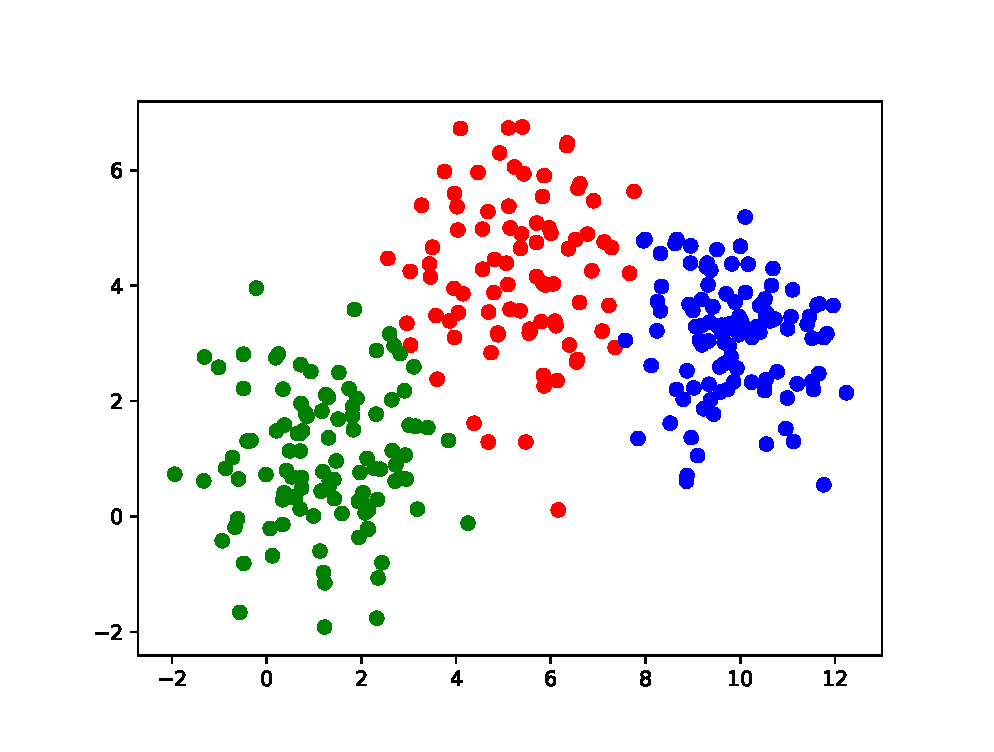
\includegraphics[width=\textwidth]{uneven.eps}
    \caption{两类椭圆形数据点}\label{fig:kmeans_wrong}
    \end{subfigure}~
    \begin{subfigure}[b]{0.45\textwidth}
    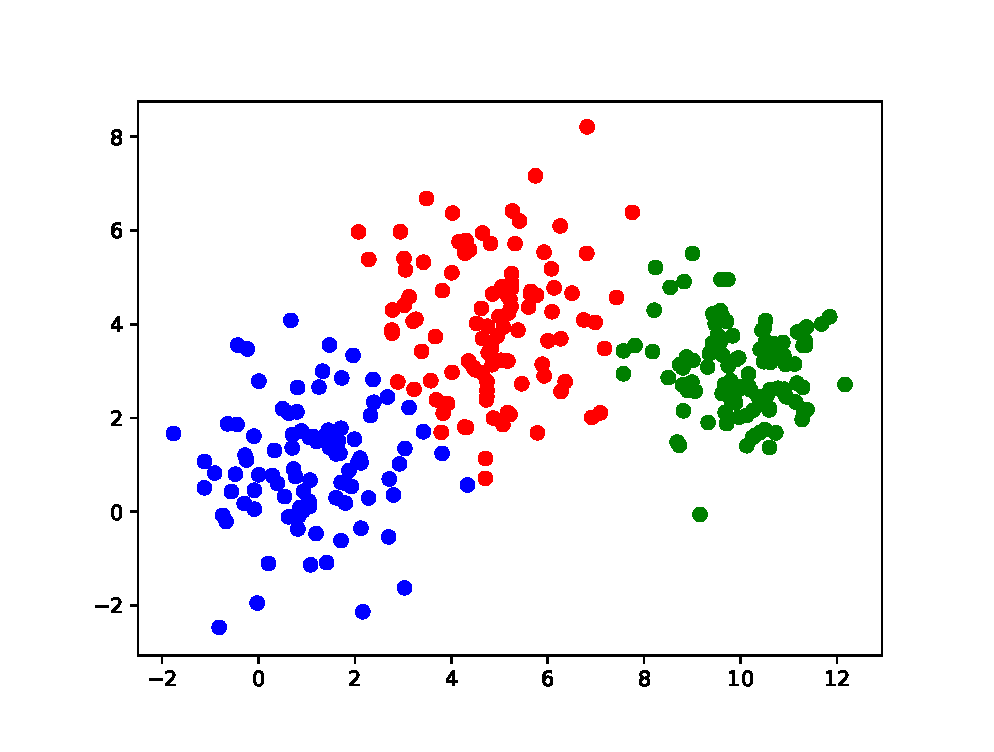
\includegraphics[width=\textwidth]{even.eps}
    \caption{三类各向同性数据点}\label{fig:kmeans_right}
    \end{subfigure}
\end{figure}

我们使用混合高斯模型产生二维数据点,针对方差矩阵非均匀的情况,受\cite{kmeans-bad} 的启发,我们做了图\ref{fig:kmeans_wrong}所示的数值实验,验证了对于非均匀的数据点
使用k-means 算法可能得到与直觉不一致的结果。

但对于通常的情形,比如图\ref{fig:kmeans_right}所示的数值实验,k-means 给出了比较合理的结果。

\begin{table}[!ht]
\centering
\begin{tabular}{ccc}
\hline
& 三类各向同性数据点 & 两类椭圆形数据点 \\
\hline
标签差异度 & 0.1\% & 6.6\% \\
目标函数相对差 & 1e-4 & 0.02 \\
平均迭代次数 & 6.2 & 11.5 \\
\hline
\end{tabular}
\caption{k-means 算法比较}\label{tb:compare}
\end{table}

根据\ref{verification}小节提出的指标,我们比较了k-means标准算法的工业级实现和自己的实现,结果如表\ref{tb:compare}所示。表\ref{tb:compare}所示的结果为30次聚类结果取平均得到的。

三类各向同性数据点是比较适合于用k-means算法进行聚类的人工数据集,其标签差异度仅为0.1\%左右,这意味着平均意义上1000个数据点有1个点两种算法聚类结果不一致,可见我们实现的算法与工业级算法在结果上的高度稳合性。目标函数相对差只有1e-4左右,说明目标函数有局部最优值,但在比较适合用k-means聚类的情形下不同实现(初值点不一样)得到的局部最优值非常接近。

两类椭圆形数据点,如图\ref{fig:kmeans_wrong}所示,是不适合用k-means进行聚类的。如果使用的话,如表\ref{tb:compare}所示,标签差异度和目标函数相对差均较大。这说明了问题对初值点比较敏感,目标函数各局部最优值相差较大,在图\ref{fig:kmeans_wrong}的$x$轴附近的数据点在不同的聚类实例中会随机地分到两个类中从而导致了总体标签差异度较大。

表\ref{tb:compare}还展示了k-means算法在实验人工数据集上的收敛速度,在比较合适的数据集上仅用6次多就收敛,而在不合适的数据集上要11.5次才收敛。

\begin{figure}[!ht]
    \centering
    \begin{subfigure}[b]{\textwidth}
    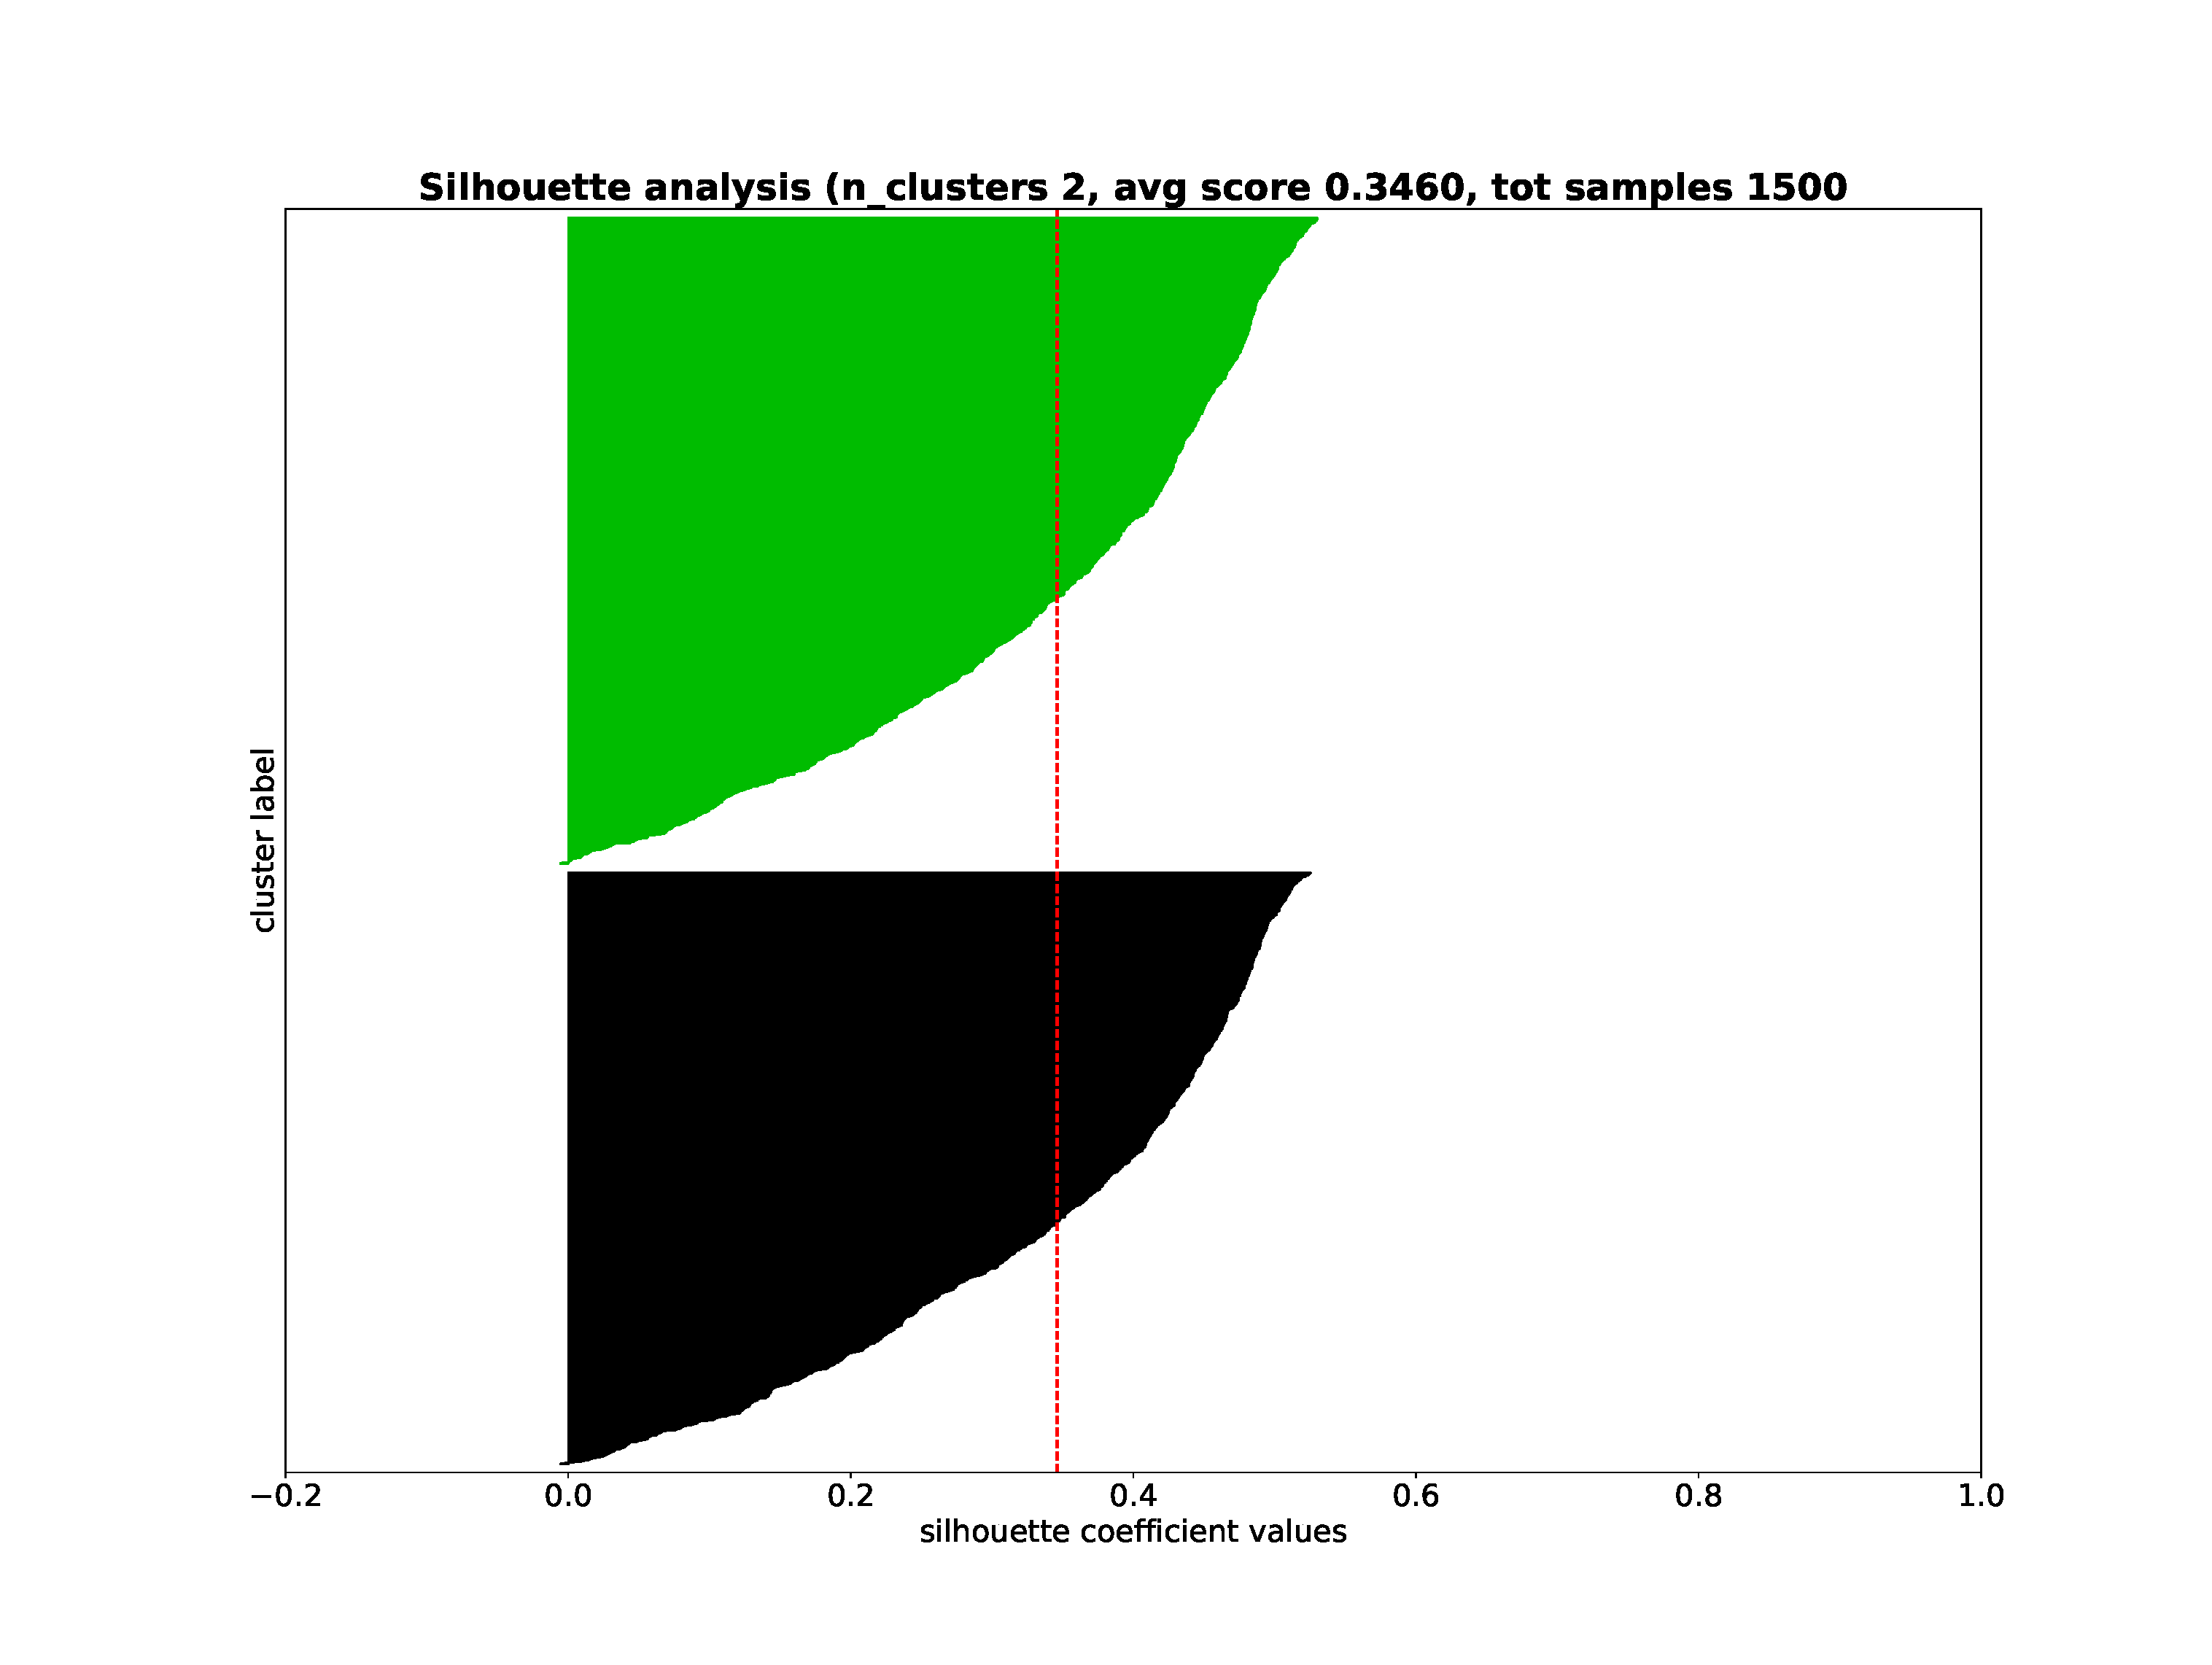
\includegraphics[height=8cm, width=\textwidth]{uneven_s.eps}
    \caption{两类椭圆形数据点}\label{fig:silhouette_uneven}
    \end{subfigure}\\
    \begin{subfigure}[b]{\textwidth}
    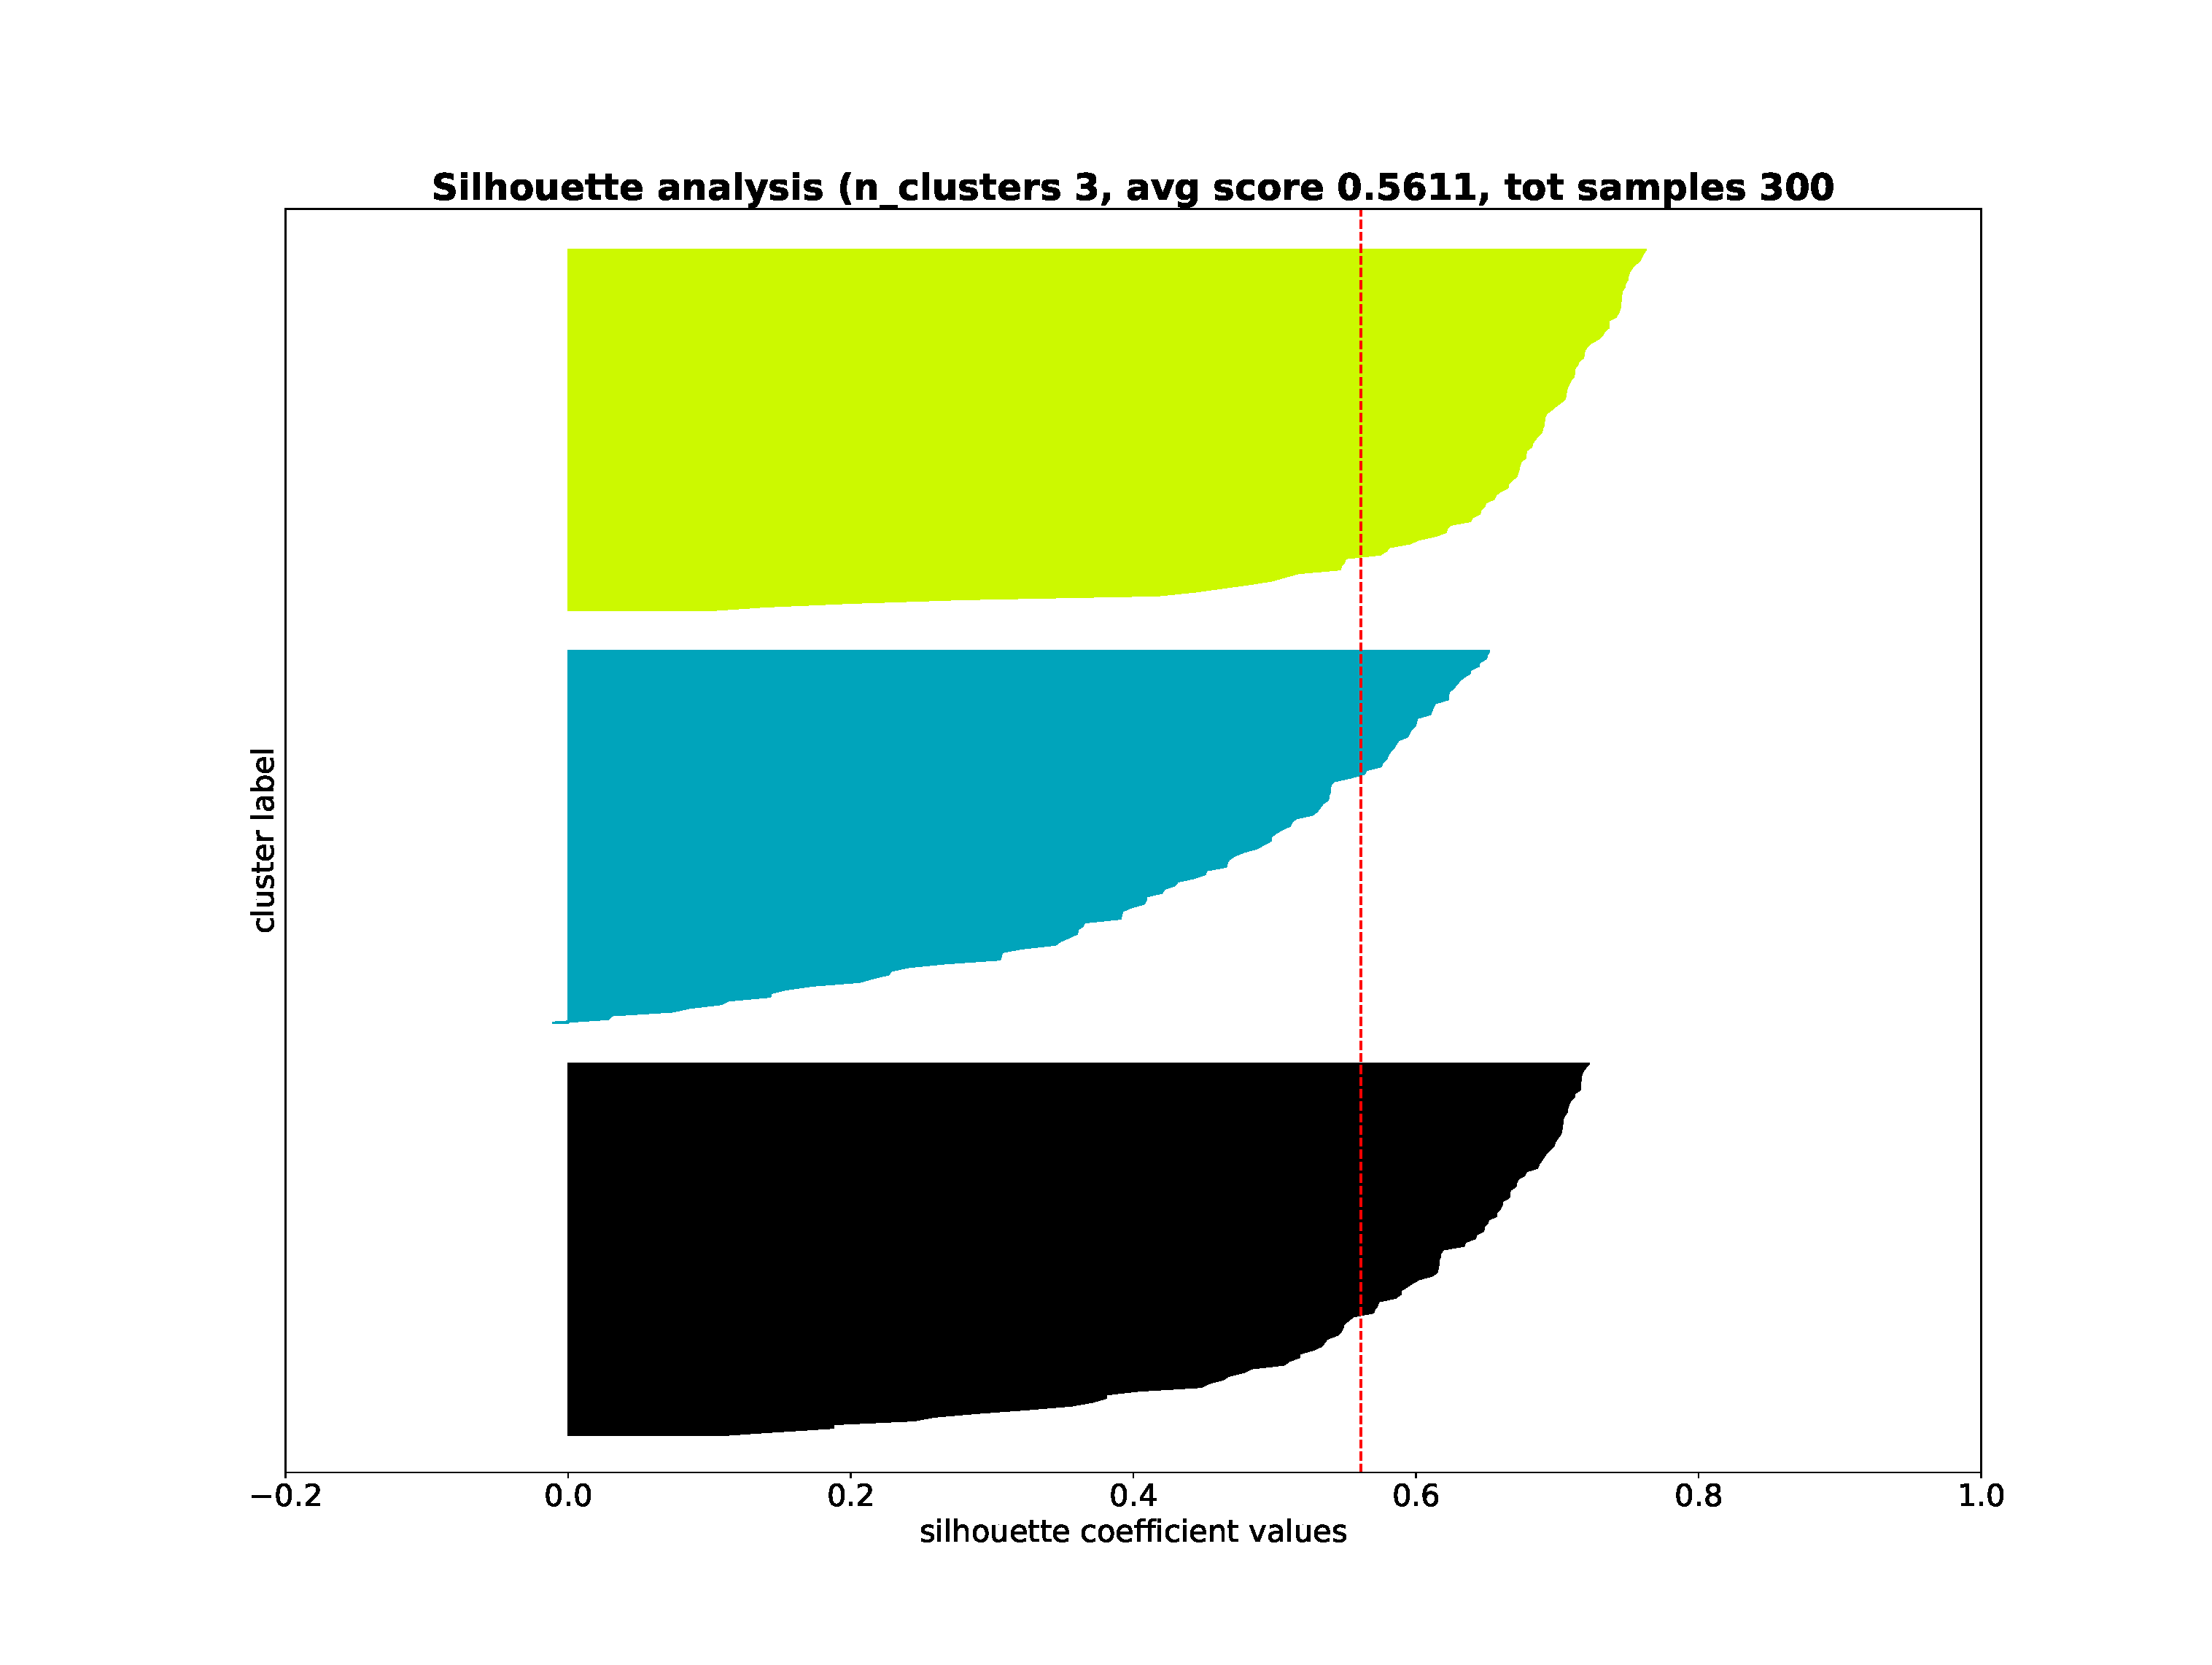
\includegraphics[height=8cm, width=\textwidth]{even_s.eps}
    \caption{三类各向同性数据点}\label{fig:silhouette_even}
    \end{subfigure}
     \caption{Silhouette 作图}\label{fig:silhouette}
\end{figure}

我们对均一和非均一两组人工数据集的k-means 聚类结果分别做出silhouette 图,如\ref{fig:silhouette_uneven}所示。 由图可见,对于两类椭圆形数据点 silhouette 值较低, 平均只有0.34,聚类效果不好;
而对于三类各向同性数据点,silhouette得分平均值为0.56,相比较而言较好。
\subsection{工业级k-means标准算法代码阅读}
通过阅读工业级k-means标准算法的源码\cite{kmeans-industry},我总结出以下算法独有的特点:
\begin{enumerate}
\item 换不同的初值点多算几次取目标函数最小的作为返回结果
\item 默认使用 k-means++ 选取初值点加快收敛速度
\item 对于稀疏矩阵和稠密矩阵区别处理
\end{enumerate}

而我实现的算法初值是随便选取的,只算一次,不考虑矩阵的稀疏性。

工业级k-means标准算法的源码对于迭代过程中可能出现的$S_i$为空(求质心不能除以零)的情况采用了\textbf{经验式}的处理方法,即取那些距现有中心最远的点单独归为一类,该点即为此类的质心。
而我在算法实现中采用不更新质心的经验式方法,即下一轮的迭代的质心就是上一轮的。
\section{Affinity Propagation 算法}
我们用 Affinity Propagation 算法对两类椭圆形数据点和三类各向同性数据点进行聚类,发现存在如下问题:
\begin{enumerate}
\item 理论时间复杂度是 $O(tdn^2)$,$t$为迭代次数,$d$为数据维数,而$n$为数据个数。实际运行结果的感受也是Affinity Propagation 远慢于 k-means 。
\item Affinity Propagation 无须事先指定聚类数$k$的个数,但个人感觉在数据看上去不是分的很开的情况下(三类各向同性数据点)默认参数$s(i,i)$产生的$k$太大,为使聚类数为3, 需要用区间搜索法调参,对不同的问题又需要重新调参,增加了计算开销。
\item Affinity Propagation 即使在有阻尼系数的情况下收敛速度可能会很慢。在两类各向同性数据点的情形下,实际测试发现将默认的最大迭代次数调节到1000时仍不能保证收敛。
\item 从分类的结果来看,对于两类各向同性数据点,产生的分类结果和k-means一致而与预期的类不一致,说明 Affinity Propagation也不能很好地处理非均匀数据分布。
\end{enumerate}
基于我们的实际测试,我们得出的结论是 Affinity Propagation 不是一个很好的算法,效率低、聚类结果差、调参繁琐,对部分问题不适用。
\section{图像分割}
对于彩色图像,其三个通道的色彩值在一定程度上代表了图像的局部特征,我们利用这一点在RGB色彩空间对给定的图片用k-means算法进行聚类,输入图像如图~\ref{fig:pepper}所示,实验结果如图~\ref{fig:segementation}所示。
\begin{figure}[!ht]
    \centering
    \begin{subfigure}[b]{\textwidth}
    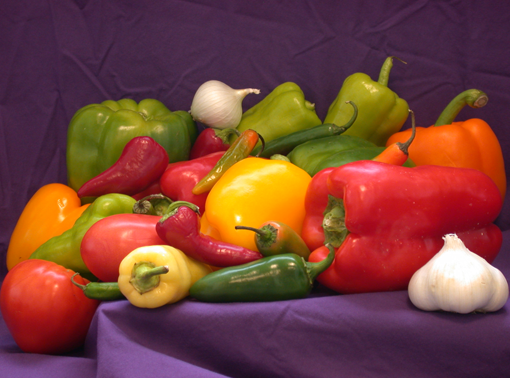
\includegraphics[height=8cm, width=\textwidth]{pepper.jpg}
    \caption{输入图像}\label{fig:pepper}
    \end{subfigure}\\
    \begin{subfigure}[b]{\textwidth}
    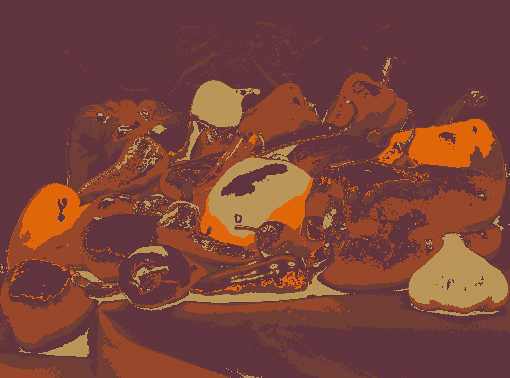
\includegraphics[height=8cm, width=\textwidth]{segementation.png}
    \caption{$k=5$ 聚类效果图}\label{fig:segementation}
    \end{subfigure}
     \caption{k-means 图像分割}
\end{figure}

通过实际测试发现存在如下问题:
\begin{enumerate}
\item 由于图像每个像素点均为一个待聚类的数据点,规模很大,即使用k-means聚类单次迭代的速度也很慢。
\item 收敛速度很慢,我们设置最大迭代次数为200次仍不收敛, 聚类效果欠佳。
\end{enumerate}
\begin{thebibliography}{9}
\bibitem{kmeans-wiki} \href{https://en.wikipedia.org/wiki/k-means_clustering}{维基百科k-means}
\bibitem{kmeans-csdn} \href{https://blog.csdn.net/zouxy09/article/details/17589329}{机器学习算法与Python实践之(五)k均值聚类(k-means)}
\bibitem{kmeans-bad} \href{http://scikit-learn.org/stable/auto_examples/cluster/plot_kmeans_assumptions.html#sphx-glr-auto-examples-cluster-plot-kmeans-assumptions-py}{Demonstration of k-means assumptions}
\bibitem{A_Multiplicative_Metric} \href{http://www.jstor.org/stable/2690124?seq=1#page_scan_tab_contents}{A Multiplicative Metric}
\bibitem{kmeans-industry}\href{https://github.com/scikit-learn/scikit-learn/blob/master/sklearn/cluster/k_means_.py}{sklearn k-means implementation}
\end{thebibliography}
\end{document}

